\section{History of AES}

The history of the Advanced Encryption Standard (AES) reflects a turning point in cryptographic development, 
addressing the weakness of the Data Encryption Standard (DES) and resulting in the selection of Rijndael as the new standard.  

\subsection{Why DES Failed and AES Was Needed}

Initially adopted in the 1970s, DES became one of the most widely used symmetric encryption algorithms. However, by the late 1990s, 
its security was more and more questioned due to its short key length of 56 bits. This key size made DES vulnerable to brute-force attacks, 
as demonstrated by projects like the Electronic Frontier Foundation's DES cracker - \textit{Deep Crack} (shown in Figure~\ref{fig:deep-crack})—which could break DES within days. 
Furthermore, DES was susceptible to various cryptanalytic techniques, including differential and linear cryptanalysis, which exploited its structural weaknesses. 
Although Triple DES (3DES) extended DES's lifespan by using multiple keys, it was computationally inefficient and unsuitable for many modern applications.  
These vulnerabilities not only compromised data integrity but also emphasized the urgent need for a more robust encryption standard that could provide 
better security and efficiency for a wide range of applications. 

\begin{figure}[h] % 'h' means place the figure here if possible
    \centering
    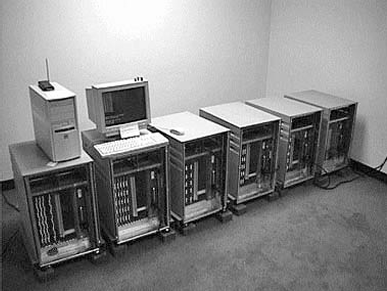
\includegraphics[width=.5\textwidth]{deep_crack.png} % Adjust width as needed
    \caption{
        Deep Crack - the hardware exhaustive key-search machine that broke DES in 1998
    }
    \label{fig:deep-crack} % Reference this figure with \ref{fig:sample_image}
\end{figure}
 

\subsection{NIST Competition and Selection Process}

To address the arising challenges, the National Institute of Standards and Technology (NIST) launched a global competition in 1997 to select a new encryption standard. 
The evaluation criteria included security strength, performance across various platforms, flexibility in supporting different key sizes, and resistance to known cryptanalytic attacks. 
After thorough discussion in the scientific community, five finalists—MARS, RC6, Serpent, Twofish, and Rijndael—were selected for further scrutiny. \newline 


Developed by Belgian cryptographers Vincent Rijmen and Joan Daemen, Rijndael was ultimately chosen as the AES algorithm due to its outstanding performance in meeting all evaluation criteria. 
It supports key sizes of 128, 192, and 256 bits while maintaining a fixed block size of 128 bits for AES. NIST officially adopted Rijndael as AES with the publication of 
Federal Information Processing Standards (FIPS) 197 in November 2001. 